% =====================================================================
% BMED365: AI and Health - Introduction
% Beamer presentation in widescreen (16:9)
% =====================================================================
\documentclass[aspectratio=169, 10pt]{beamer}

% =====================================================================
% PACKAGES
% =====================================================================
\usepackage[utf8]{inputenc}
\usepackage[T1]{fontenc}
\usepackage[english]{babel}
\usepackage{graphicx}
\usepackage{tikz}
\usetikzlibrary{shapes.geometric, arrows, positioning, shapes.symbols}
\usepackage{booktabs}
\usepackage{amsmath}
\usepackage{fontawesome5}
\usepackage{hyperref}
\hypersetup{colorlinks=true, linkcolor=blue, urlcolor=blue}

% =====================================================================
% THEME AND COLORS
% =====================================================================
\usetheme{Madrid}
\usecolortheme{beaver}

% Colors for TikZ diagrams
\definecolor{uibblue}{RGB}{0, 61, 115}
\definecolor{uibred}{RGB}{175, 28, 44}

% =====================================================================
% TITLE INFO
% =====================================================================
\title{AI and Health -- Introduction}
\subtitle{BMED365: What is AI, History, and AI/ML/DL Concepts}
\author{BMED365}
\date{Spring 2026}

% =====================================================================
% DOCUMENT
% =====================================================================
\begin{document}

% ---------------------------------------------------------------------
% Title slide
% ---------------------------------------------------------------------
\begin{frame}
    \titlepage
\end{frame}

% ---------------------------------------------------------------------
% Overview
% ---------------------------------------------------------------------
\begin{frame}{Overview}
    \begin{enumerate}
        \item \textbf{What is Artificial Intelligence?}
        \begin{itemize}
            \item Definition of AI
            \item Narrow vs. General AI
            \item The Turing Test
            \item AI in everyday life and healthcare
        \end{itemize}
        \item \textbf{AI in Healthcare: A Historical Journey}
        \begin{itemize}
            \item Timeline: 1950s to today
            \item Key milestones and systems
            \item Lessons from history
            \item Future perspectives
        \end{itemize}
        \item \textbf{AI, ML, and DL: Understanding the Terminology}
        \begin{itemize}
            \item Hierarchical relationship
            \item Machine Learning fundamentals
            \item Deep Learning and neural networks
            \item Decision guide: Which approach to choose?
        \end{itemize}
    \end{enumerate}
\end{frame}

% =====================================================================
\section{What is Artificial Intelligence?}
% =====================================================================

% ---------------------------------------------------------------------
% Definition of AI
% ---------------------------------------------------------------------
\begin{frame}{What is Artificial Intelligence?}

    \begin{block}{\footnotesize Definition}
        \footnotesize
        \textbf{Artificial Intelligence (AI)} are systems that can:
        \begin{itemize}
            \item Solve tasks that normally require human intelligence
            \item Learn from experience
            \item Adapt to new situations
            \item Reason and make decisions
        \end{itemize}
    \end{block}

    \vspace{2mm}
    \begin{columns}
        \begin{column}{0.48\textwidth}
            \textbf{Examples of AI:}
            \begin{itemize}
                \item Google Maps route finding
                \item Automatic text translation
                \item Facial recognition
                \item Spam filters
            \end{itemize}
        \end{column}
        \begin{column}{0.48\textwidth}
            \textbf{NOT AI:}
            \begin{itemize}
                \item Simple calculator
                \item Thermostat
                \item Database storage
            \end{itemize}
        \end{column}
    \end{columns}

\end{frame}

% ---------------------------------------------------------------------
% Narrow vs General AI
% ---------------------------------------------------------------------
\begin{frame}{Narrow vs. General AI}

    \begin{columns}
        \begin{column}{0.48\textwidth}
            \textbf{\faBullseye\ Narrow AI (ANI):}
            \begin{itemize}
                \item Designed for specific tasks
                \item All current AI is narrow AI
                \item Examples:
                \begin{itemize}
                    \item Chess AI
                    \item Image recognition
                    \item Language translation
                \end{itemize}
            \end{itemize}
        \end{column}

        \begin{column}{0.48\textwidth}
            \textbf{\faGlobe\ General AI (AGI):}
            \begin{itemize}
                \item Can solve any intellectual task
                \item Human-like intelligence
                \item Doesn't exist yet
                \item (Maybe never will?)
            \end{itemize}

            \vspace{3mm}
            \textbf{\faRocket\ Superintelligence (ASI):}
            \begin{itemize}
                \item Surpasses human intelligence
                \item Science fiction (for now!)
            \end{itemize}
        \end{column}
    \end{columns}

    \vspace{3mm}
    \begin{center}
        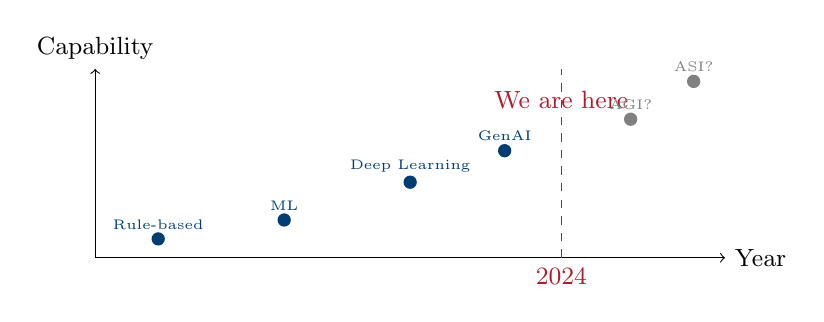
\begin{tikzpicture}[scale=0.8]
            \draw[->] (0,0) -- (10,0) node[right] {\small Year};
            \draw[->] (0,0) -- (0,3) node[above] {\small Capability};
            
            % Mark current position
            \draw[dashed, uibred] (7.4,0) -- (7.4,3);
            \node[uibred] at (7.4, -0.3) {\small 2024};
            \node[uibred] at (7.4, 2.5) {\small We are here};
            
            % Mark milestones
            \fill[uibblue] (1,0.3) circle (3pt) node[above] {\tiny Rule-based};
            \fill[uibblue] (3,0.6) circle (3pt) node[above] {\tiny ML};
            \fill[uibblue] (5,1.2) circle (3pt) node[above] {\tiny Deep Learning};
            \fill[uibblue] (6.5,1.7) circle (3pt) node[above] {\tiny GenAI};
            \fill[gray] (8.5,2.2) circle (3pt) node[above] {\tiny AGI?};
            \fill[gray] (9.5,2.8) circle (3pt) node[above] {\tiny ASI?};
        \end{tikzpicture}
    \end{center}

\end{frame}

% ---------------------------------------------------------------------
% The Turing Test
% ---------------------------------------------------------------------
\begin{frame}{The Turing Test: Can Machines Think?}

    \begin{block}{\footnotesize Alan Turing (1950)}
        \footnotesize
        A person chats with both a human and a machine. If the person cannot tell them apart $\rightarrow$ The machine is ``intelligent''.
    \end{block}

    \vspace{3mm}
    \begin{columns}
        \begin{column}{0.48\textwidth}
            \textbf{AI Response:}
            \begin{itemize}
                \item Structured, fact-based
                \item Professional tone
                \item Consistent
            \end{itemize}
            \textit{``Based on the symptoms, this could be tension headache. Common triggers include stress, dehydration, and poor sleep.''}
        \end{column}

        \begin{column}{0.48\textwidth}
            \textbf{Human Response:}
            \begin{itemize}
                \item Personal anecdotes
                \item Emotional language
                \item Less formal
            \end{itemize}
            \textit{``Oh, headaches can be so annoying! I remember when I had migraines... Have you tried lying in a dark room?''}
        \end{column}
    \end{columns}

    \vspace{3mm}
    \begin{alertblock}{\footnotesize Relevance for Healthcare}
        \footnotesize
        The Turing Test raises questions about AI's role in patient communication and whether AI can truly understand human needs.
    \end{alertblock}

\end{frame}

% ---------------------------------------------------------------------
% AI in Healthcare
% ---------------------------------------------------------------------
\begin{frame}{AI in Healthcare Today}

    \begin{columns}
        \begin{column}{0.48\textwidth}
            \textbf{Healthcare Areas:}
            \begin{itemize}
                \item \textbf{Diagnostics:} Image analysis (X-ray, MRI)
                \item \textbf{Treatment:} Robotic surgery, medication optimization
                \item \textbf{Administration:} Medical records, scheduling
                \item \textbf{Research:} Drug development, genomics
                \item \textbf{Monitoring:} Wearables, remote monitoring
                \item \textbf{Prevention:} Risk prediction, health apps
            \end{itemize}
        \end{column}

        \begin{column}{0.48\textwidth}
            \begin{center}
                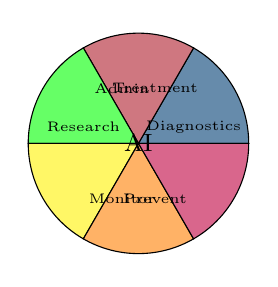
\begin{tikzpicture}[scale=0.7]
                    % Pie chart representation
                    \draw[fill=uibblue!60] (0,0) -- (0:2) arc (0:60:2) -- cycle;
                    \draw[fill=uibred!60] (0,0) -- (60:2) arc (60:120:2) -- cycle;
                    \draw[fill=green!60] (0,0) -- (120:2) arc (120:180:2) -- cycle;
                    \draw[fill=yellow!60] (0,0) -- (180:2) arc (180:240:2) -- cycle;
                    \draw[fill=orange!60] (0,0) -- (240:2) arc (240:300:2) -- cycle;
                    \draw[fill=purple!60] (0,0) -- (300:2) arc (300:360:2) -- cycle;
                    
                    \node at (0,0) {\small AI};
                    \node at (1,0.3) {\tiny Diagnostics};
                    \node at (0.3,1) {\tiny Treatment};
                    \node at (-0.3,1) {\tiny Admin};
                    \node at (-1,0.3) {\tiny Research};
                    \node at (-0.3,-1) {\tiny Monitor};
                    \node at (0.3,-1) {\tiny Prevent};
                \end{tikzpicture}
            \end{center}
        \end{column}
    \end{columns}

    \vspace{3mm}
    \begin{block}{\footnotesize Strengths of Today's AI}
        \footnotesize
        Processes large amounts of data quickly, finds patterns humans overlook, consistent performance 24/7, can be specialized for specific tasks.
    \end{block}

\end{frame}

% =====================================================================
\section{AI in Healthcare: A Historical Journey}
% =====================================================================

% ---------------------------------------------------------------------
% Timeline Overview
% ---------------------------------------------------------------------
\begin{frame}{AI in Healthcare: Historical Timeline}

    \begin{columns}
        \begin{column}{0.48\textwidth}
            \textbf{1950-1980: Foundation}
            \begin{itemize}
                \item 1950: Turing Test
                \item 1966: ELIZA (therapy chatbot)
                \item 1972: MYCIN (antibiotic system)
                \item 1976: INTERNIST-I
            \end{itemize}

            \vspace{2mm}
            \textbf{1980-2010: Expert Systems}
            \begin{itemize}
                \item 1986: DXplain launched
                \item 1995: Robot-assisted surgery
            \end{itemize}
        \end{column}

        \begin{column}{0.48\textwidth}
            \textbf{2010-Today: AI Revolution}
            \begin{itemize}
                \item 2012: Deep Learning breakthrough
                \item 2016: AlphaGo defeats Go master
                \item 2018: FDA approves AI for diabetic retinopathy
                \item 2020: COVID-19 accelerates AI adoption
                \item 2023: ChatGPT and generative AI
            \end{itemize}
        \end{column}
    \end{columns}

    \vspace{3mm}
    \begin{center}
        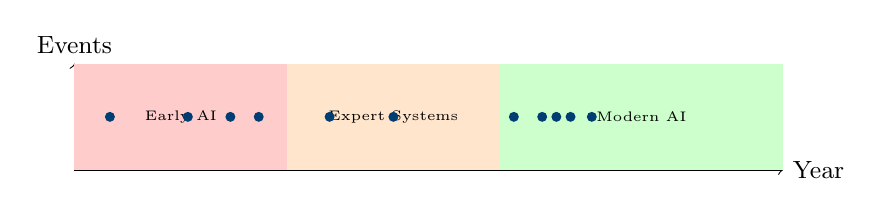
\begin{tikzpicture}[scale=0.9]
            \draw[->] (0,0) -- (10,0) node[right] {\small Year};
            \draw[->] (0,0) -- (0,1.5) node[above] {\small Events};
            
            % Time periods
            \fill[red!20] (0,0) rectangle (3,1.5);
            \fill[orange!20] (3,0) rectangle (6,1.5);
            \fill[green!20] (6,0) rectangle (10,1.5);
            
            \node at (1.5, 0.75) {\tiny Early AI};
            \node at (4.5, 0.75) {\tiny Expert Systems};
            \node at (8, 0.75) {\tiny Modern AI};
            
            % Mark events
            \foreach \x/\label in {0.5/1950, 1.6/1966, 2.2/1972, 2.6/1976, 3.6/1986, 4.5/1995, 6.2/2012, 6.6/2016, 6.8/2018, 7/2020, 7.3/2023} {
                \fill[uibblue] (\x, 0.75) circle (2pt);
            }
        \end{tikzpicture}
    \end{center}

\end{frame}

% ---------------------------------------------------------------------
% Key Milestones
% ---------------------------------------------------------------------
\begin{frame}{Key Milestones: Early Systems}

    \begin{columns}
        \begin{column}{0.32\textwidth}
            \textbf{1950: Turing Test}
            \begin{itemize}
                \item Foundation for assessing AI
                \item Still relevant today
            \end{itemize}

            \vspace{2mm}
            \textbf{1966: ELIZA}
            \begin{itemize}
                \item First ``therapist chatbot''
                \item Simulated Rogerian psychotherapist
                \item Showed potential and limitations
            \end{itemize}
        \end{column}

        \begin{column}{0.32\textwidth}
            \textbf{1972: MYCIN}
            \begin{itemize}
                \item Expert system for antibiotics
                \item Diagnosed bacterial infections
                \item Performed as well as experts
            \end{itemize}

            \vspace{2mm}
            \textbf{1976: INTERNIST-I}
            \begin{itemize}
                \item Comprehensive diagnostic system
                \item Handled thousands of diseases
                \item Demonstrated complexity
            \end{itemize}
        \end{column}

        \begin{column}{0.32\textwidth}
            \textbf{1986: DXplain}
            \begin{itemize}
                \item First commercial medical expert system
                \item Still in use today (updated)
                \item Shows importance of continuous development
            \end{itemize}

            \vspace{2mm}
            \textbf{1995: Robot-assisted surgery}
            \begin{itemize}
                \item da Vinci system introduced
                \item Revolutionized precision
                \item Combined AI with robotics
            \end{itemize}
        \end{column}
    \end{columns}

\end{frame}

% ---------------------------------------------------------------------
% Modern AI Revolution
% ---------------------------------------------------------------------
\begin{frame}{Modern AI Revolution (2010-Today)}

    \begin{columns}
        \begin{column}{0.48\textwidth}
            \textbf{2012: Deep Learning Breakthrough}
            \begin{itemize}
                \item CNNs win ImageNet
                \item Starts modern AI revolution
                \item Opens advanced medical image analysis
            \end{itemize}

            \vspace{2mm}
            \textbf{2016: AlphaGo}
            \begin{itemize}
                \item Defeats world champion in Go
                \item Demonstrates strategic thinking
                \item Inspires complex medical decision-making
            \end{itemize}
        \end{column}

        \begin{column}{0.48\textwidth}
            \textbf{2018: FDA Approval}
            \begin{itemize}
                \item First autonomous AI system approved
                \item IDx-DR for diabetic retinopathy
                \item Milestone for AI as medical device
            \end{itemize}

            \vspace{2mm}
            \textbf{2020: COVID-19}
            \begin{itemize}
                \item AI accelerates vaccine development
                \item Rapid diagnosis from imaging
                \item Demonstrates AI's value in crises
            \end{itemize}

            \vspace{2mm}
            \textbf{2023: Generative AI}
            \begin{itemize}
                \item ChatGPT and similar models
                \item New possibilities for medical writing
                \item Paradigm shift in AI interaction
            \end{itemize}
        \end{column}
    \end{columns}

\end{frame}

% ---------------------------------------------------------------------
% Lessons from History
% ---------------------------------------------------------------------
\begin{frame}{Lessons from History}

    \begin{columns}
        \begin{column}{0.48\textwidth}
            \textbf{\faCheckCircle\ Success Factors:}
            \begin{enumerate}
                \item \textbf{Specialization first:} Early systems like MYCIN focused on narrow domains
                \item \textbf{Iterative improvement:} DXplain continuously evolved since 1986
                \item \textbf{Regulatory approval:} FDA process ensures safety
                \item \textbf{Crises as catalyst:} COVID-19 accelerated adoption
            \end{enumerate}
        \end{column}

        \begin{column}{0.48\textwidth}
            \textbf{\faExclamationTriangle\ Challenges and Failures:}
            \begin{enumerate}
                \item \textbf{Over-optimism:} Many early systems promised more than delivered
                \item \textbf{User acceptance:} Physicians were skeptical
                \item \textbf{Integration:} Difficult to integrate into workflows
                \item \textbf{Responsibility:} Who is responsible when AI makes mistakes?
            \end{enumerate}
        \end{column}
    \end{columns}

    \vspace{3mm}
    \begin{block}{\footnotesize Key Insight}
        \footnotesize
        AI is powerful, but requires thoughtfulness, testing, and gradual implementation. History shows that successful AI systems are those that solve specific problems well and evolve over time.
    \end{block}

\end{frame}

% ---------------------------------------------------------------------
% Future Perspectives
% ---------------------------------------------------------------------
\begin{frame}{Future Perspectives: Next 5-10 Years}

    \begin{columns}
        \begin{column}{0.48\textwidth}
            \textbf{Expected Developments:}
            \begin{itemize}
                \item \textbf{Multimodal AI:} Combining text, images, sensors
                \item \textbf{Personalized medicine:} AI tailored to individuals
                \item \textbf{Real-time monitoring:} Continuous health monitoring
                \item \textbf{Robotics:} Advanced surgical and care robots
            \end{itemize}

            \vspace{2mm}
            \textbf{Expected AI Maturity (2024 $\rightarrow$ 2030):}
            \begin{itemize}
                \item Medical image diagnostics: 7/10 $\rightarrow$ 9/10
                \item Drug development: 4/10 $\rightarrow$ 8/10
                \item Patient monitoring: 5/10 $\rightarrow$ 8/10
                \item Surgical assistance: 3/10 $\rightarrow$ 7/10
            \end{itemize}
        \end{column}

        \begin{column}{0.48\textwidth}
            \textbf{Challenges Ahead:}
            \begin{itemize}
                \item \textbf{Data quality and bias:} Ensure representative datasets
                \item \textbf{Interoperability:} AI systems that communicate
                \item \textbf{Ethics and regulation:} Balance innovation with safety
                \item \textbf{Education:} Prepare healthcare personnel
            \end{itemize}

            \vspace{3mm}
            \begin{alertblock}{\footnotesize The Future}
                \footnotesize
                AI will transform all aspects of healthcare, but requires careful implementation and ethical considerations.
            \end{alertblock}
        \end{column}
    \end{columns}

\end{frame}

% =====================================================================
\section{AI, ML, and DL: Understanding the Terminology}
% =====================================================================

% ---------------------------------------------------------------------
% Hierarchical Relationship
% ---------------------------------------------------------------------
\begin{frame}{AI, ML, and DL: The Hierarchical Relationship}

    \begin{center}
        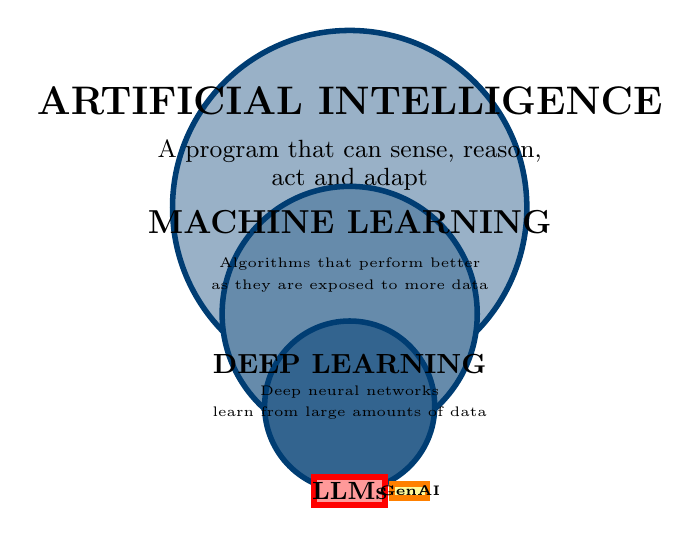
\begin{tikzpicture}[scale=0.9]
            % AI circle (largest, top)
            \draw[fill=uibblue!40, draw=uibblue, line width=2pt] (0,2) circle (2.5cm);
            \node[font=\Large\bfseries] at (0, 3.5) {ARTIFICIAL INTELLIGENCE};
            \node[font=\small] at (0, 2.8) {A program that can sense, reason,};
            \node[font=\small] at (0, 2.4) {act and adapt};

            % ML circle (medium, middle)
            \draw[fill=uibblue!60, draw=uibblue, line width=2pt] (0,0.5) circle (1.8cm);
            \node[font=\large\bfseries] at (0, 1.8) {MACHINE LEARNING};
            \node[font=\tiny] at (0, 1.2) {Algorithms that perform better};
            \node[font=\tiny] at (0, 0.9) {as they are exposed to more data};

            % DL circle (smallest, bottom)
            \draw[fill=uibblue!80, draw=uibblue, line width=2pt] (0,-0.8) circle (1.2cm);
            \node[font=\normalsize\bfseries] at (0, -0.2) {DEEP LEARNING};
            \node[font=\tiny] at (0, -0.6) {Deep neural networks};
            \node[font=\tiny] at (0, -0.9) {learn from large amounts of data};

            % LLMs box
            \draw[fill=red!40, draw=red, line width=2pt] (-0.5, -1.8) rectangle (0.5, -2.2);
            \node[font=\small\bfseries] at (0, -2) {LLMs};

            % GenAI box
            \draw[fill=yellow!40, draw=orange, line width=2pt] (0.6, -1.9) rectangle (1.1, -2.1);
            \node[font=\tiny\bfseries] at (0.85, -2) {GenAI};
        \end{tikzpicture}
    \end{center}

    \vspace{2mm}
    \begin{block}{\footnotesize Key Point}
        \footnotesize
        \textbf{Deep Learning $\subseteq$ Machine Learning $\subseteq$ Artificial Intelligence}
        
        LLMs (Large Language Models) and Generative AI are the newest areas within deep learning.
    \end{block}

\end{frame}

% ---------------------------------------------------------------------
% Machine Learning Fundamentals
% ---------------------------------------------------------------------
\begin{frame}{Machine Learning: From Mystery to Mathematics}

    \begin{block}{\footnotesize The Machine Learning Formula}
        \footnotesize
        \[ y \approx f(x; \theta) \]
        \begin{itemize}
            \item $x$ = Input (data: table, text, image, audio, \ldots)
            \item $f$ = Model (function/algorithm)
            \item $\theta$ = Model parameters (learned from data)
            \item $y$ = Output (diagnosis, prognosis, grade, type, \ldots)
        \end{itemize}
    \end{block}

    \vspace{2mm}
    \begin{columns}
        \begin{column}{0.48\textwidth}
            \textbf{Why Mathematics?}
            \begin{itemize}
                \item \textbf{Clarity:} Precise understanding
                \item \textbf{Communication:} Speak with colleagues
                \item \textbf{Problem Solving:} Debug and improve
            \end{itemize}
        \end{column}

        \begin{column}{0.48\textwidth}
            \textbf{Why ``$\approx$'' not ``$=$''?}
            \begin{itemize}
                \item Models give approximations
                \item Always uncertainty and error
                \item In healthcare: ``85\% probability of diabetes'', not ``definitely diabetes''
            \end{itemize}
        \end{column}
    \end{columns}

    \vspace{2mm}
    \begin{alertblock}{\footnotesize Important}
        \footnotesize
        AI results must always be interpreted with caution! The symbol $\approx$ reminds us that predictions are probabilistic, not deterministic.
    \end{alertblock}

\end{frame}

% ---------------------------------------------------------------------
% Types of Machine Learning
% ---------------------------------------------------------------------
\begin{frame}{Types of Machine Learning}

    \begin{columns}
        \begin{column}{0.32\textwidth}
            \textbf{\faCheckCircle\ Supervised Learning:}
            \begin{itemize}
                \item Data has \textbf{labels}
                \item Learn input$\rightarrow$output mapping
                \item Types: Classification, regression
                \item Medical: Diagnosis, prognosis
            \end{itemize}

            \vspace{2mm}
            \begin{center}
                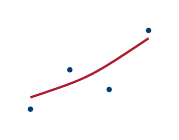
\begin{tikzpicture}[scale=0.5]
                    \fill[uibblue] (0,0) circle (2pt);
                    \fill[uibblue] (1,1) circle (2pt);
                    \fill[uibblue] (2,0.5) circle (2pt);
                    \fill[uibblue] (3,2) circle (2pt);
                    \draw[uibred, thick] (0,0.3) .. controls (1.5,0.8) .. (3,1.8);
                \end{tikzpicture}
            \end{center}
        \end{column}

        \begin{column}{0.32\textwidth}
            \textbf{\faSearch\ Unsupervised Learning:}
            \begin{itemize}
                \item Data \textbf{without} labels
                \item Finds hidden patterns
                \item Types: Clustering, dimensionality reduction
                \item Medical: Patient subgroups
            \end{itemize}

            \vspace{2mm}
            \begin{center}
                \begin{tikzpicture}[scale=0.5]
                    \fill[uibblue] (0.5,0.5) circle (2pt);
                    \fill[uibblue] (0.8,1) circle (2pt);
                    \fill[uibblue] (1,0.7) circle (2pt);
                    \fill[uibred] (2,2) circle (2pt);
                    \fill[uibred] (2.3,1.8) circle (2pt);
                    \fill[uibred] (1.8,2.2) circle (2pt);
                \end{tikzpicture}
            \end{center}
        \end{column}

        \begin{column}{0.32\textwidth}
            \textbf{\faTrophy\ Reinforcement Learning:}
            \begin{itemize}
                \item Environment with reward/punishment
                \item Optimize actions
                \item Medical: Medication dosing optimization
            \end{itemize}

            \vspace{2mm}
            \begin{center}
                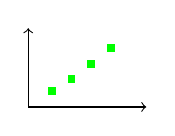
\begin{tikzpicture}[scale=0.5]
                    \draw[->] (0,0) -- (3,0);
                    \draw[->] (0,0) -- (0,2);
                    \fill[green] (0.5,0.3) rectangle (0.7,0.5);
                    \fill[green] (1,0.6) rectangle (1.2,0.8);
                    \fill[green] (1.5,1) rectangle (1.7,1.2);
                    \fill[green] (2,1.4) rectangle (2.2,1.6);
                \end{tikzpicture}
            \end{center}
        \end{column}
    \end{columns}

\end{frame}

% ---------------------------------------------------------------------
% Deep Learning
% ---------------------------------------------------------------------
\begin{frame}{Deep Learning: ML with Neural Networks}

    \begin{block}{\footnotesize Definition}
        \footnotesize
        \textbf{Deep Learning} is a subset of machine learning that uses neural networks with many layers (``deep'' networks) to learn complex patterns.
    \end{block}

    \vspace{2mm}
    \begin{columns}
        \begin{column}{0.48\textwidth}
            \textbf{Characteristics:}
            \begin{itemize}
                \item Neural networks with many layers
                \item Automatic feature engineering
                \item Handles complex data (images, text, audio)
                \item Requires large amounts of data and computing power
            \end{itemize}

            \vspace{2mm}
            \textbf{Deep Learning Architectures:}
            \begin{itemize}
                \item \textbf{CNN:} Images (X-ray analysis)
                \item \textbf{RNN:} Sequences (ECG interpretation)
                \item \textbf{Transformer:} Language (medical report writing)
                \item \textbf{GAN:} Generation (synthetic medical images)
            \end{itemize}
        \end{column}

        \begin{column}{0.48\textwidth}
            \begin{center}
                \begin{tikzpicture}[scale=0.6]
                    % Simple neural network visualization
                    % Input layer
                    \foreach \y in {0,1,2} {
                        \fill[uibblue] (0,\y) circle (0.15);
                    }
                    \node[left] at (-0.3, 1) {\tiny Input};
                    
                    % Hidden layer 1
                    \foreach \y in {0,0.5,1,1.5,2} {
                        \fill[uibblue] (2,\y) circle (0.15);
                    }
                    \node at (2, -0.3) {\tiny Hidden 1};
                    
                    % Hidden layer 2
                    \foreach \y in {0.3,0.8,1.3,1.7} {
                        \fill[uibblue] (4,\y) circle (0.15);
                    }
                    \node at (4, -0.3) {\tiny Hidden 2};
                    
                    % Output layer
                    \foreach \y in {0.5,1.5} {
                        \fill[uibblue] (6,\y) circle (0.15);
                    }
                    \node[right] at (6.3, 1) {\tiny Output};
                    
                    % Connections
                    \foreach \y1 in {0,1,2} {
                        \foreach \y2 in {0,0.5,1,1.5,2} {
                            \draw[gray, very thin] (0.15,\y1) -- (1.85,\y2);
                        }
                    }
                    \foreach \y1 in {0,0.5,1,1.5,2} {
                        \foreach \y2 in {0.3,0.8,1.3,1.7} {
                            \draw[gray, very thin] (2.15,\y1) -- (3.85,\y2);
                        }
                    }
                    \foreach \y1 in {0.3,0.8,1.3,1.7} {
                        \foreach \y2 in {0.5,1.5} {
                            \draw[gray, very thin] (4.15,\y1) -- (5.85,\y2);
                        }
                    }
                \end{tikzpicture}
            \end{center}
            \vspace{2mm}
            \textit{Each layer learns more complex patterns}
        \end{column}
    \end{columns}

\end{frame}

% ---------------------------------------------------------------------
% Personalized Medicine
% ---------------------------------------------------------------------
\begin{frame}{Deep Learning: The Future of Personalized Medicine}

    \begin{block}{\footnotesize Vision from E. Topol (Nature Medicine, 2019)}
        \footnotesize
        Deep learning can revolutionize healthcare by combining \textbf{all available data} about a patient into \textbf{individualized treatment}.
    \end{block}

    \vspace{2mm}
    \begin{columns}
        \begin{column}{0.48\textwidth}
            \textbf{Input (x) - Multimodal data:}
            \begin{itemize}
                \item Genomics (DNA, RNA, proteins)
                \item Clinical data (lab values, vital signs)
                \item Lifestyle (activity, sleep, diet)
                \item Cognitive state
                \item Medical literature
                \item Biosensors (real-time data)
            \end{itemize}
        \end{column}

        \begin{column}{0.48\textwidth}
            \textbf{Output (y) - Personalized guidance:}
            \begin{itemize}
                \item Precise diagnosis
                \item Tailored treatment
                \item Optimal timing
                \item Prognosis
            \end{itemize}

            \vspace{2mm}
            \textbf{Why Revolutionary?}
            \begin{itemize}
                \item Holistic approach
                \item Individualization
                \item Continuous improvement
                \item Prevention focus
            \end{itemize}
        \end{column}
    \end{columns}

    \vspace{2mm}
    \begin{alertblock}{\footnotesize Challenges}
        \footnotesize
        Data quality, privacy, interpretability, bias, regulation. Still a future vision, but pilot projects are underway.
    \end{alertblock}

\end{frame}

% ---------------------------------------------------------------------
% Comparison of Approaches
% ---------------------------------------------------------------------
\begin{frame}{Comparison: When Do We Use What?}

    \begin{table}
        \centering
        \footnotesize
        \begin{tabular}{lccc}
            \toprule
            \textbf{Aspect} & \textbf{Rule-based} & \textbf{Traditional ML} & \textbf{Deep Learning} \\
            \midrule
            Data volume & Low & Medium & High \\
            Interpretability & High & Medium & Low \\
            Computing power & Low & Medium & High \\
            Development time & Short & Medium & Long \\
            Accuracy (complex data) & Low & Medium & High \\
            \bottomrule
        \end{tabular}
    \end{table}

    \vspace{3mm}
    \begin{columns}
        \begin{column}{0.48\textwidth}
            \textbf{Healthcare Examples:}
            \begin{itemize}
                \item \textbf{Rule-based:} Medication dosing, allergy alerts
                \item \textbf{Traditional ML:} Risk scores, patient grouping
                \item \textbf{Deep Learning:} Image analysis, language processing
            \end{itemize}
        \end{column}

        \begin{column}{0.48\textwidth}
            \textbf{Case Study: X-ray Analysis}
            \begin{itemize}
                \item \textbf{Rule-based:} 60-70\% accuracy
                \item \textbf{Traditional ML:} 75-85\% accuracy
                \item \textbf{Deep Learning:} 90-95\% accuracy
            \end{itemize}
        \end{column}
    \end{columns}

\end{frame}

% ---------------------------------------------------------------------
% Decision Guide
% ---------------------------------------------------------------------
\begin{frame}{Decision Guide: Which Approach Should I Choose?}

    \begin{block}{\footnotesize Answer These Questions:}
        \footnotesize
        \begin{enumerate}
            \item \textbf{How much data do you have?}
            \begin{itemize}
                \item Little ($<$ 1000) $\rightarrow$ Rule-based
                \item Moderate (1000-100k) $\rightarrow$ Traditional ML
                \item A lot ($>$ 100k) $\rightarrow$ Can consider Deep Learning
            \end{itemize}
            \item \textbf{How important is interpretability?}
            \begin{itemize}
                \item Critical (medical diagnosis) $\rightarrow$ Rule-based or interpretable ML
                \item Important $\rightarrow$ Traditional ML
                \item Less important $\rightarrow$ Deep Learning OK
            \end{itemize}
        \end{enumerate}
    \end{block}

    \vspace{2mm}
    \begin{block}{\footnotesize More Questions:}
        \footnotesize
        \begin{enumerate}
            \setcounter{enumi}{2}
            \item \textbf{How complex are your data?}
            \begin{itemize}
                \item Simple (numbers, categories) $\rightarrow$ Rule-based/Traditional ML
                \item Complex (images, text, audio) $\rightarrow$ Deep Learning
            \end{itemize}
            \item \textbf{How much time/resources do you have?}
            \begin{itemize}
                \item Limited $\rightarrow$ Rule-based
                \item Moderate $\rightarrow$ Traditional ML
                \item Good resources $\rightarrow$ Deep Learning
            \end{itemize}
        \end{enumerate}
    \end{block}

    \vspace{2mm}
    \begin{alertblock}{\footnotesize Recommendation}
        \footnotesize
        \textbf{ALWAYS start simple!} Build baseline first, then improve. Deep learning only if you really need it. A simple system that works $>$ complex system that doesn't work.
    \end{alertblock}

\end{frame}

% ---------------------------------------------------------------------
% Summary
% ---------------------------------------------------------------------
\begin{frame}{Summary: Key Points}

    \begin{columns}
        \begin{column}{0.32\textwidth}
            \textbf{\footnotesize What is AI?}
            \scriptsize
            \begin{itemize}\setlength{\itemsep}{0pt}
                \item Systems that solve tasks requiring human intelligence
                \item Narrow AI (current) vs. General AI (future)
                \item Turing Test: Can machines think?
                \item AI in everyday life and healthcare
            \end{itemize}
        \end{column}

        \begin{column}{0.32\textwidth}
            \textbf{\footnotesize AI History}
            \scriptsize
            \begin{itemize}\setlength{\itemsep}{0pt}
                \item 1950s: Foundation (Turing, ELIZA, MYCIN)
                \item 1980s-2000s: Expert systems (DXplain, robotics)
                \item 2010s: Deep Learning revolution
                \item 2020s: Generative AI and multimodal systems
                \item Lessons: Specialization, iteration, regulation
            \end{itemize}
        \end{column}

        \begin{column}{0.34\textwidth}
            \textbf{\footnotesize AI/ML/DL Concepts}
            \scriptsize
            \begin{itemize}\setlength{\itemsep}{0pt}
                \item DL $\subseteq$ ML $\subseteq$ AI (hierarchical)
                \item ML: $y \approx f(x; \theta)$
                \item Supervised/Unsupervised/Reinforcement
                \item Deep Learning: Neural networks with many layers
                \item Decision guide: Start simple!
            \end{itemize}
        \end{column}
    \end{columns}

    \vspace{3mm}
    \begin{block}{\footnotesize Practical Advice}
        \footnotesize
        \textbf{Start simple} -- build baseline first. \textbf{Consider data volume} -- more data = more complex methods. \textbf{Think interpretability} -- critical in medicine. \textbf{Resources} -- deep learning requires time and computing power.
    \end{block}

    \vspace{2mm}
    \begin{center}
        \textbf{\large Thank you! Questions?}
    \end{center}

\end{frame}

\end{document}
